\chapter{Konzept zur Visualisierung von Schmerz Scores aus akustischen Signalen}

In Kapitel \ref{sec:medicalFoundations} wurde vorgestellt, wie die Schmerzdiagnose bei Neugeborenen mit Hilfe von Pain Scales durch medizinisches Personal durchgeführt wird. Es wurde eine Reihe an Pain Scales vorgestellt und dabei insbesondere der Schmerzindikator \glqq Weinen\grqq{} beleuchtet. Unabhängig von der konkret eingesetzten Pain Scale wird in jedem Fall das Baby für eine bestimme Zeitraum beobachtet, für jeden Indikator, wie das Weinen oder der Gesichtsausdruck, Punkte vergeben, diese Aufsummiert und aus der Summe der insgesamte Schmerz Score bestimmt. 

In Kapitel \ref{sec:cryresearch_foundations} wurde vorgestellt, wie in der klassischen Schreiforschung mit Hilfe von Methoden der Signalverarbeitung das Weinen von Babys tiefergehend Analysiert wurde. Es wurde gezeigt, dass aus objektiv messbaren Eigenschaften des Weinens eines Babys Rückschlüsse auf dessen Zustand gemacht werden können.

Ziel dieser Arbeit ist der Entwurf eines Systems zur automatisierten Feststellung und Visualisierung von Pain Scores beliebiger Pain Scales mit dem Fokus auf den Schmerzindikator \glqq Weinen\grqq. Das System muss folgenden Anforderungen erfüllen:

\begin{enumerate}
	\item Das System muss dazu in der Lage sein, aus den akustischen Eigenschaften des Weinens eines Babys den Schmerz Score bezüglich einer Pain Scale abzuleiten.
	\item Das System muss dazu in der Lage sein, die abgeleiteten Schmerz Scores zu visualisieren.
	\item Das System muss dazu in der Lage sein, beliebige Pain Scales einzubinden. 
	\item Die System muss dazu in der Lage sein, die Analyse auch bei nicht-optimalen akustischen Bedingungen durchzuführen.
	\item Das System muss dazu in der Lage sein, die Analyse kontinuierlich durchzuführen.
\end{enumerate}

Der \textbf{Input} des Systems ist folglich ein Audiosignal, welches kontinuierlich in das System gegeben wird. Der \textbf{Output} ist eine Visualisierung der abgeleiteten Pain Score, welche kontinuierlich erzeugt wird.

In Kapitel \ref{sec:system_literature} wird zunächst ein Überblick über einige Veröffentlichungen gegeben, in denen Konzepte zur automatisierten Analyse und Auswertung kindlicher Lautäußerungen vorgestellt wurden. In Kapitel \ref{sec:pipeline} wird daraufhin das in dieser Arbeit entworfene Konzept in Form einer Verarbeitungs-Pipeline vorgestellt. Diese Verarbeitungs-Pipeline kombiniert das Vorgehen bei der Schmerzdiagnostik auf Basis der Pain Scales, Methoden der klassischen Schreiforschung sowie einige Ideen der im folgenden Kapitel vorgestellten Veröffentlichungen.

\section{Literaturüberblick}
\label{sec:system_literature}

Der größere Teil der Veröffentlichungen, die sich in das Feld der Analyse von Audioaufnahmen Neugeborener einordnen lassen, stellten Algorithmen zur Klassifizierung einzelner Cry Units vor, entweder bezüglich der Weinursache (Hunger, Angst, Schmerz, ... ) oder zur Diagnose bestimmter Krankheiten. Diese Methoden waren in den meisten Fällen nicht für die kontinuierliche Analyse geeignet, sondern hatten das Ziel, eine gegebenen Cry-Unit mit einer möglichst hohen Genauigkeit bezüglich des jeweiligen Sachverhaltes zu klassifizieren. Probleme wie Hintergrundrauschen, Berechnungsaufwand oder kontextuelle Informationen haben eine untergeordnete Rolle gespielt. Beispiele für solche Veröffentlichungen sind die von Abdulaziz et al. \cite{class_abdulaziz} oder Fuhr et al. \cite{comparisonOfLearning}.

Várallyay stellte in seiner Dissertation \glqq Analysis of the Infant Cry with Objective Methods\grqq{} \cite{cry_thesis} Methoden zur automatisierten Analyse kindlicher Lautäußerungen vor. Das primäre Ziel der Dissertation war die Erforschung der Unterschiede zwischen den Lautäußerungen gesunder und tauber Neugeborener. Die Algorithmen zur automatisierten Analyse der Audiosignale waren ein \glqq Nebenprodukt\grqq{} zur schnelleren Datenauswertung. Die Auswertung musste nicht kontinuierlich erfolgen. In der vorgestellten Verarbeitungs-Pipeline wurde das Eingangssignal in Zeitfenster weniger Millisekunden zerlegt und jedes Fenster nach Entscheidungsregeln als \emph{stimmhaft} oder \emph{nicht stimmhaft} markiert. Die stimmhaften Signalfenster wurden zu \emph{Segmenten} zusammengefasst (welche in Kapitel \ref{sec:acousticModel} als Cry-Units bezeichnet werden). Auf Basis der Segmente wurden Auswertungen bezüglich des Zeitbereiches (Durchschnittliche Segmentlänge, Pausenlängen etc.), des Frequenzbereiches (Grund-Frequenz, Formanten-Frequenzen etc.) und des Melodieverlaufes angestellt. Analysiert wurden Audioaufnahmen von Babys mit einer Länge von 10 bis \SI{100}{\second}. Aus den Auswertungsergebnisse stellte Varallyay die wichtigsten Unterscheidungsmerkmale zwischen tauben und gesunden Babys fest. In der Dissertation \cite{cry_thesis} wird ein Überblick über das Vorgehen und die Ergebnisse gegeben. Die Verarbeitungsschritte wurden detaillierter in einzelnen Veröffentlichungen beschrieben, wobei der Autor dieser Arbeit nur den Zugriff auf einige dieser Veröffentlichungen erhalten konnte.

Cohen et al. haben 2012 in der Veröffentlichung \glqq Infant Cry Analysis and Detection\grqq{} \cite{cohenCry}  ein System zur Analyse der akustischen Signale von Neugeborenen vorgestellt. Dieses System klassifizierte die Audiosignale in eine der drei Klassen \emph{Cry, No Cry} und \emph{No Activity}. Die Klasse \emph{Cry} bezeichnet Lautäußerungen, die eine potentiell Gefahr für das Baby anzeigen, wie z.B. wie Schmerz oder Hunger. Die Klasse \emph{No Cry} bedeutete, dass das Baby zwar Laute von sich gibt, diese aber keine potentielle Gefahr anzeigen. Die Klasse \emph{No Activity} bezeichnete keinerlei Lautäußerung. Die Verarbeitungs-Pipeline wurde detailliert vorgestellt und war für die kontinuierliche Verarbeitung mit einer gewissen Verzögerungszeit spezialisiert. Das Signal wird in überlappende \emph{Segmente} \`{a} \SI{10}{\second} zerlegt. Die Stimmaktivität in den Segmenten wird algorithmisch festgestellt. Wenn Aktivität vorliegt, wird das Segment in Sektionen \`{a} \SI{1}{\second} zerlegt und die Stimmaktivität für jede Sektion gemessen. Wird genügend Stimmaktivität in einer Sektion festgestellt, wird die Sektion in \emph{Frames} \`{a} \SI{32}{\milli\second} zerlegt und Attribute für jeden Frame errechnet. Mit Hilfe von Entscheidungsregeln werden die Frames in \emph{Cry, No-Cry} oder \emph{No Activity} klassifiziert, wobei kontextuelle Informationen der umliegenden Frames mit einbezogen werden. Aus den Klassen der Frames wird auf die Klasse der Sektion geschlossen, und aus den Klassen der Sektionen auf die Klasse des Segmentes. Das System hat mit den Anforderungen dieser Arbeit gemeinsam, dass ebenfalls die kontinuierliche Verarbeitung im Vordergrund steht. Der Nachteil an dieser Methode ist, dass die zeitliche längste Einheit, für die die Klassifizierung vorgenommen wird, unflexibel auf \SI{10}{\second} festgelegt ist. Daher müsste diese Verarbeitungs-Pipeline abgewandelt werden, um anstelle der Ableitung der drei genannten Klassen einen Pain Score ableiten zu können, die einen längeren Beobachtungszeitraum als \SI{10}{\second} benötigt.

Pal et al.  haben 2006 in der Veröffentlichung \glqq Emotion detection from infant facial experessions and cries\grqq{} \cite{palEmotion} ein System vorgestellt, welches aus den akustischen Eigenschaften des Weinens die Emotion ableitet. Die zu erkennenden Emotionen sind \emph{Traurigkeit, Wut, Hunger, Angst und Schmerz}. Es wird nicht erwähnt, ob die Analyse kontinuierlich oder nicht kontinuierlich erfolgt. Bei der Verarbeitung der akustischen Signale werden die Attribute \emph{Grundtonhöhe} und die \emph{Frequenz der ersten drei Formanten} extrahiert und mit einem Klassifizierungsalgorithmus klassifiziert. Es wurde nicht beschrieben, inwiefern die Eigenschaften aus kurzen Signalfenstern oder längeren Signalabschnitten errechnet werden, welche Vorverarbeitungsschritte angewandt werden und ob die Klassifizierung auf Ebene der Signalfenster oder über längere Zeitabschnitte hinweg geschieht.

Zamzi et al.  haben 2016 in der Veröffentlichung \glqq An Approach for Automated Multimodal Analysis of Infants' Pain\grqq{} \cite{zamziMultimodal} ein System zur automatisierten und kontinuierlichen multimodalen Analyse von Neugeborenen zur Ableitung des Schmerzes vorgestellt. Das System trägt den Namen \emph{MPAS}. Der Schmerzgrad wird aus den Analyseergebnissen der monomodalen Schmerzindikatoren für \emph{Gesichtsausdruck, Körperbewegung, Vitalfunktionen und Weinen} errechnet. Das System kommt der Aufgabenstellung dieser Masterarbeit am nächsten, da es ebenfalls um die Ableitung von Schmerz in einem multimodalen Verbund geht. Der Schmerz wurde hier \glqq direkt\grqq{} abgeleitet, ohne den Weg über Pain Scales zu wählen. Während in der Veröffentlichung die Analyse der ersten drei genannten Schmerzindikatoren angekündigt wurde, wurden daraufhin die Methoden zur Analyse der akustischen Signale \emph{nicht} erläutert. Auch die ersten Validierungsergebnisse beziehen sich nur auf den Gesichtsausdruck, die Körperbewegung und die Vitalfunktionen. Es ist nicht klar, ob die Miteinbeziehung akustischer Signale fallen gelassen wurde. Die Ausführungen konzentrieren sich dazu vermehrt auf die Methoden zur Kombination der Auswertungsergebnisse der monomodalen Schmerzindikatoren.

\section{Verarbeitungs-Pipeline}
\label{sec:pipeline}

In Kapitel \ref{sec:system_literature} wurden verschiedene Konzepte vorgestellt, deren Fokus ebenfalls die Analyse und Auswertung von Audioaufnahmen kindlicher Lautäußerungen waren und somit der Aufgabenstellung dieser Arbeit ähneln. Keines der präsentierten Konzepte eignet sich, um mit nur leichten Anpassungen übernommen werden zu können: Entweder wurden die Verarbeitungsschritte nicht für die kontinuierliche Verarbeitung konzipiert \cite{class_abdulaziz} \cite{comparisonOfLearning} \cite{cry_thesis}, nicht genügen abstrahiert, um für andere Klassifizierungen als die ursprünglich geplanten abgewandelt werden zu können \cite{cohenCry}, oder die Verarbeitungs-Pipeline wurde nicht vorgestellt. \cite{palEmotion} \cite{zamziMultimodal}.

In dieser Arbeit wurde die folgende Verarbeitungs-Pipeline entworfen. Sie wird in in Abbildung \ref{img:architecture-overview} visualisiert. 

%To Do: Kapitel hinzufügen.
\begin{enumerate}[leftmargin=*]
	\item \textbf{Input: } Ein Audiosignal, das möglicherweise kindliche Lautäußerungen enthält. Es wird kontinuierlich in das System gegeben.
	
	\item \textbf{Erkennung der Cry-Units}. Zunächst muss festgestellt werden, ob und wo in dem Signal kindliche Lautäußerungen vorhanden sind. Ein Algorithmus zur Feststellung von Stimmaktivität, bezeichnet als Voice Activity Detection, untersucht das Signal und markiert Cry-Units. Die gefunden Cry-Units bilden die Grundlage aller darauf folgenden Verarbeitungsschritte. Der vorgestellte Algorithmus kombinierte herkömmliche Methoden der Voice Activity Detection mit Ideen, die von Varallyay \cite{cry_thesis} vorgestellt wurden.
	
	\item \textbf{Segmentierung} (engl \emph{Segmenting}). Eine Pain Score wird nicht aus der Beobachtung einer einzigen, sondern einer Reihe von Cry-Units abgeleitet. In Kapitel \ref{sec:painScores} wurde gezeigt, dass bestimmte Pain Scores die Beobachtung über mehrere Minuten hinweg erfordern. Zu diesem Zweck werden die Cry-Units gruppiert. Da keines der in Kapitel \ref{sec:system_literature} vorgestellten Konzepte Methoden zur Segmentierung einführte, wurde ein eigener Algorithmus für diese Aufgabe entworfen.
	
	\item \textbf{Extrahierung von Eigenschaften und Ableitung der Schmerz Score} (engl. \emph{Feature Extraction} und \emph{Prediction of Pain Score}). Für jedes Segment werden Eigenschaften bezüglich des Weinens berechnet, wie zum Beispiel die durchschnittliche Tonhöhe, durchschnittliche Pausenlänge usw. Dabei werden Ideen der in Kapitel \ref{sec:cryresearch_foundations} vorgestellten klassischen Schreiforschung implementiert. Auf Basis dieser Eigenschaften wird die Pain Score abgeleitet.
	
	\item \textbf{Output: Visualisierung} (engl. \emph{Visualisation}) der abgeleiteten Schmerz Score. Es werden mehrere Varianten vorgeschlagen, bei der die Höhe des Schmerz Score in seinem zeitlichen Verlauf auf Ampelfarben abgebildet wird.
\end{enumerate}

\begin{figure}[H]
	\centering
	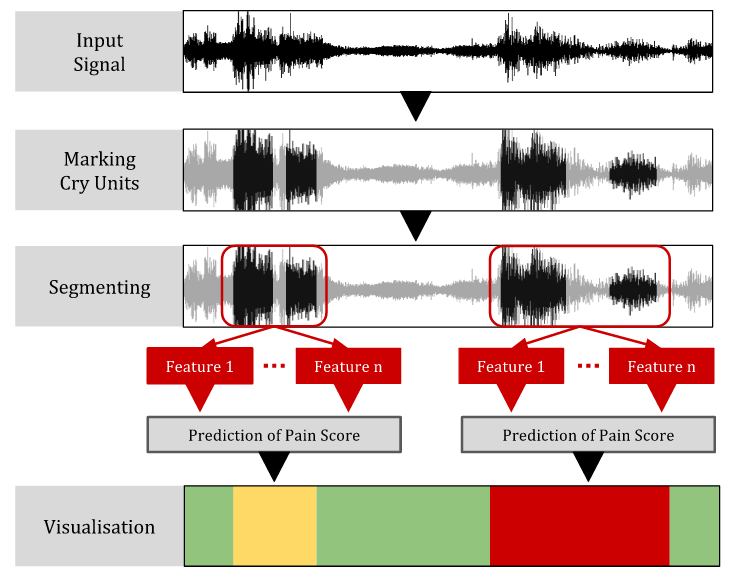
\includegraphics[width=0.75\textwidth]{bilder/konzept02.png}
	\caption{Überblick über die Verarbeitungs-Pipeline dieser Arbeit}
	\label{img:architecture-overview}
\end{figure}